\chapter{Extrapolation of difference quotients}

\section{The algorithm}

Let \(a\in \R\), \(\varepsilon > 0\) and \(f:]a - \varepsilon, a + \varepsilon [ \rightarrow \R\) be differentiable at \(a\). We are interested in estimating \(f'(a)\). Assume that \(f\) is \(2k+1\) times differentiable at \(a\). Then by Taylor's theorem we have 
\begin{equation}\label{taylor}
f(a + h) = f(a) + f'(a)h + \frac{f''(a)}{2}h^2 + \cdots + \frac{f^{(2k)}(a)}{(2k)!}h^{2k} + \frac{f^{(2k+1)}(\xi)}{(2k+1)!}h^{2k+1}
\end{equation}
where \(a < \xi < a + h\). Now plug \(-h\) instead of \(h\) in (\ref{taylor}):
\begin{equation}\label{taylorm}
f(a-h) = f(a) - f'(a)h + \frac{f''(a)}{2}h^2 - \cdots + \frac{f^{(2k)}(a)}{(2k)!}h^{2k} -  \frac{f^{(2k+1)}(\eta)}{(2k+1)!}h^{2k+1}
\end{equation}
where \(a - h < \eta < a\). If we subtract (\ref{taylorm}) from (\ref{taylor}) and divide by \(2h\) we get:
\begin{equation}\label{middlestep}
f'(a) = D_f(h) + \frac{f'''(a)}{3!}h^2 + \cdots + \frac{f^{(2k-1)}(a)}{(2k-1)!}h^{2k-2} + \frac{f^{(2k+1)}(\xi) + f^{(2k+1)}(\eta)}{2\cdot (2k+1)!}h^{2k}
\end{equation}
where
\begin{equation}
D_f(h) \coloneqq \frac{f(a+h) - f(a-h)}{2h}
\end{equation}
is the {\it symmetric difference quotient} of \(f\) at \(a\). Note that \(\frac{1}{2}(f^{(2k+1)}(\xi) + f^{(2k+1)}(\eta))\) is in the image of \(f^{(2k+1)}\) so we can rewrite (\ref{middlestep}) as 
\begin{equation}\label{symmdiff}
f'(a) = D_f(h) + \frac{f'''(a)}{3!}h^2 + \cdots + \frac{f^{(2k-1)}(a)}{(2k-1)!}h^{2k-2} + \frac{f^{(2k+1)}(\zeta)}{(2k+1)!}h^{2k}
\end{equation}
where \(a-h < \zeta < a + h\). Formula (\ref{symmdiff}) tells us that the symmetric difference quotient method has asymptotic expansion in \(h^2\) of order \(2k-2\) if \(f\) is \(2k+1\) times differentiable. Thus we can use the following scheme to extrapolate the symmetric difference quotient method:

\begin{enumerate}
    \item \(D_{i1} \coloneqq D_f(h_i)\) for \(i = 1,\ldots,k\).
    \item \(D_{ij} \coloneqq D_{i,j-1} + \frac{D_{i,j-1} - D_{i-1,j-1}}{\left(\frac{h_{i-j+1}}{h_i}\right)^2 - 1}\) for \(2\leq j\leq i\).
\end{enumerate}

\section{Numerical experiments}

In this section we are going to extrapolate the symmetric difference quotient for approximating the derivative of a function at a given point. Let \(h > 0\) be some number, \(f: ]a-\varepsilon, a+\varepsilon[\rightarrow \R\) a function differentiable at \(a\) and \(n_1 < n_2 < \cdots\) a sequence of integers. Let \(h_i \coloneqq h/n_i\). Let \(D_{ij}\) be the extrapolation table that we get from extrapolating in \(h^2\) using the points \((h_1^2,D_f(h_1)),(h_2^2,D_f(h_2)),\ldots\), as we described in the first chapter. We let \(\varepsilon_i \coloneqq |X_{ii} - f'(a)|\). We want to analyze how \(\varepsilon_i\) as \(i\) increases and we also want to do similar efficiency analyzis as in the chapter on Romberg quadrature and check whether we have exponential convergence. We will do the computations with precision up to \(500\) significant digits and also using standard double precision arithmetic.\\

Now we will consider the results of the experiments.

\subsection{The exponential function}

We begin by considering the derivative of the exponential function at zero. 

\begin{figure}[H]
\centering
\begin{minipage}{0.45\textwidth}
\centering
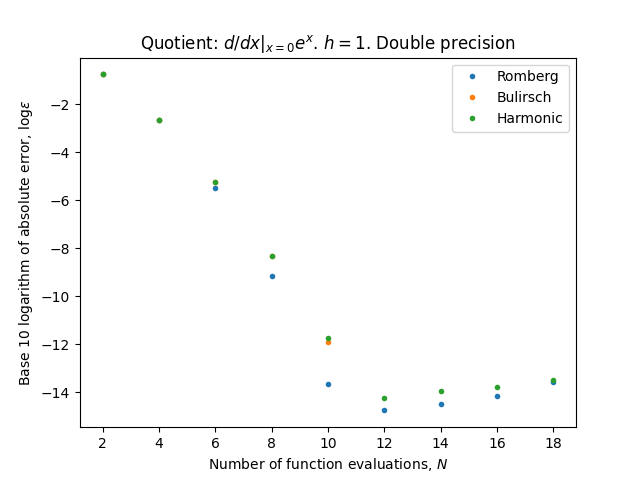
\includegraphics[scale=0.45]{diff_quot_plots/exp_0.png}
\end{minipage}
\begin{minipage}{0.45\textwidth}
\centering
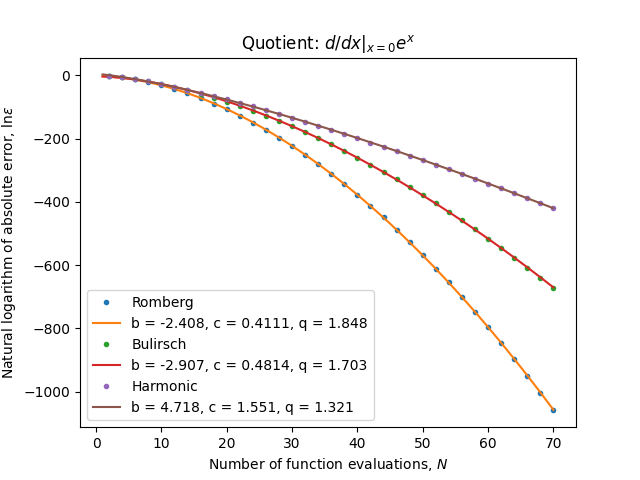
\includegraphics[scale=0.45]{diff_quot_plots/exp_0_hp_trend.png}
\end{minipage}
\end{figure}

\begin{table}[H]
    \centering
    \small
    \begin{tabular}{c|c||c|c|c|c|c|c}
Sequence & Plot & \(A\)-mean & \(A\)-var & \(c\)-mean & \(c\)-var & \(q\)-mean & \(q\)-var\\\hline
Romberg & lin-ln evals-error & \(0.1079\) & \(3.508\) & \(0.4046\) & \(0.01413\) & \(1.85\) & \(0.0002493\) \\
Bulirsch & lin-ln evals-error & \(0.08951\) & \(4.763\) & \(0.463\) & \(0.04109\) & \(1.712\) & \(0.0008086\) \\
Harmonic & lin-ln evals-error & \(4.149\cdot 10^{6}\) & \(6.499\) & \(1.734\) & \(0.02291\) & \(1.303\) & \(0.000902\) \\
    \end{tabular}
    \label{tab:my_label}
\end{table}

In standard floating point arithmetic, we get down to machine level precision using any sequence. The Romberg sequence works best, then Bulirsch and then the harmonic. The model fits moderately well for the Bulirsch and harmonic sequence but quite well for the Romberg sequence.

\subsection{Logarithm}

Now we will consider the dervative at zero of the function 
\[
g_a(x) \coloneqq \ln(x+a), \quad a > 0.
\]

\begin{figure}[H]
\centering
\begin{minipage}{0.45\textwidth}
\centering
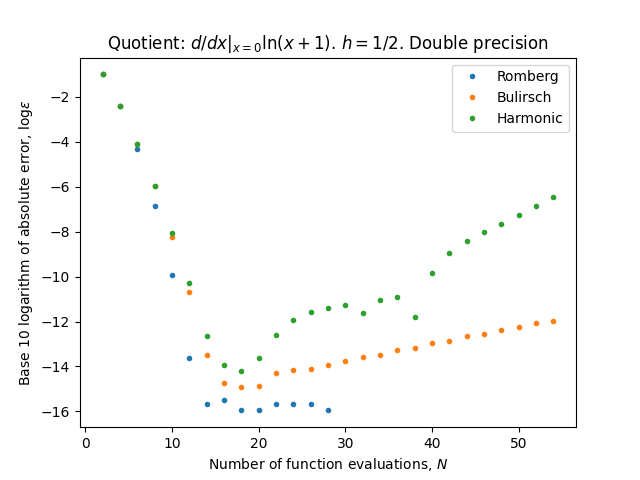
\includegraphics[scale=0.45]{diff_quot_plots/h_one.png}
\end{minipage}
\begin{minipage}{0.45\textwidth}
\centering
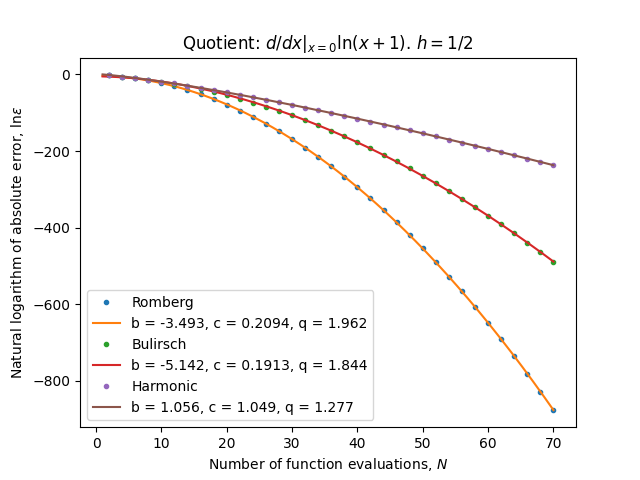
\includegraphics[scale=0.45]{diff_quot_plots/h_one_hp_trend.png}
\end{minipage}
\end{figure}

\begin{table}[H]
    \centering
    \small
    \begin{tabular}{c|c||c|c|c|c|c|c}
Sequence & Plot & \(A\)-mean & \(A\)-var & \(c\)-mean & \(c\)-var & \(q\)-mean & \(q\)-var\\\hline
Romberg & lin-ln evals-error & \(0.01503\) & \(2.443\) & \(0.2078\) & \(0.007242\) & \(1.962\) & \(0.000123\) \\
Bulirsch & lin-ln evals-error & \(0.005981\) & \(6.275\) & \(0.1873\) & \(0.08379\) & \(1.851\) & \(0.001315\) \\
Harmonic & lin-ln evals-error & \(96.18\) & \(2.331\) & \(1.128\) & \(0.01092\) & \(1.264\) & \(0.0004176\) \\
    \end{tabular}
    \label{tab:my_label}
\end{table}

We get down to machine level precision using any sequence, Romberg performes best, then Bulirsch and then the Harmonic one. The model fits quite well for the Romberg sequence and the Harmonic one, but not so well for Bulirsch.

\begin{figure}[H]
\centering
\begin{minipage}{0.45\textwidth}
\centering
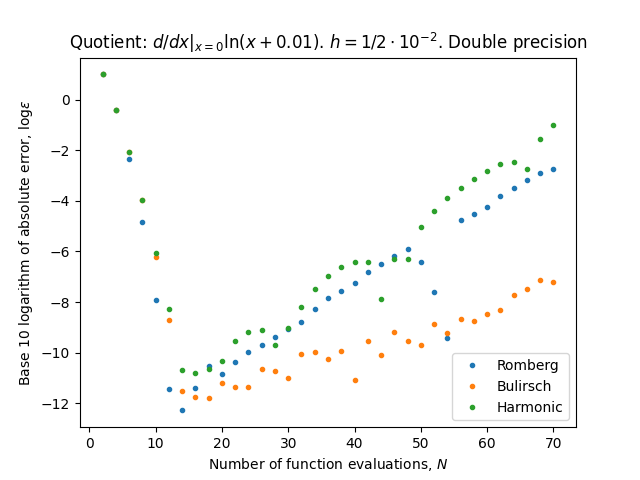
\includegraphics[scale=0.45]{diff_quot_plots/h_hundredth.png}
\end{minipage}
\begin{minipage}{0.45\textwidth}
\centering
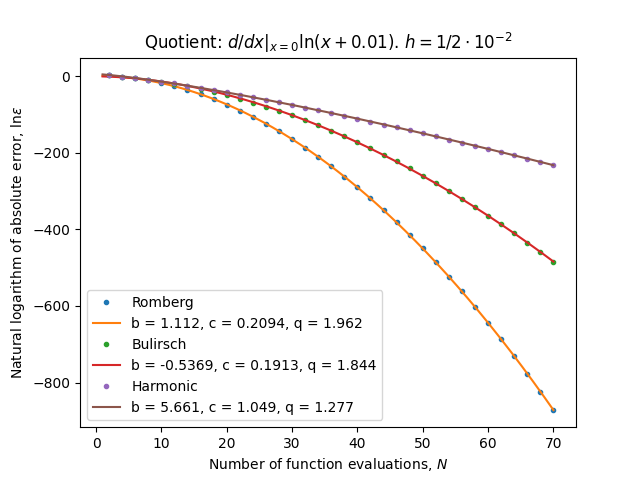
\includegraphics[scale=0.45]{diff_quot_plots/h_hundredth_hp_trend.png}
\end{minipage}
\end{figure}

\begin{table}[H]
    \centering
    \small
    \begin{tabular}{c|c||c|c|c|c|c|c}
Sequence & Plot & \(A\)-mean & \(A\)-var & \(c\)-mean & \(c\)-var & \(q\)-mean & \(q\)-var\\\hline
Romberg & lin-ln evals-error & \(1.503\) & \(2.443\) & \(0.2078\) & \(0.007242\) & \(1.962\) & \(0.000123\) \\
Bulirsch & lin-ln evals-error & \(0.5981\) & \(6.275\) & \(0.1873\) & \(0.08379\) & \(1.851\) & \(0.001315\) \\
Harmonic & lin-ln evals-error & \(9618\) & \(2.331\) & \(1.128\) & \(0.01092\) & \(1.264\) & \(0.0004176\) \\
    \end{tabular}
    \label{tab:my_label}
\end{table}

Here the same comments apply as for \(a = 1\).

\begin{figure}[H]
\centering
\begin{minipage}{0.45\textwidth}
\centering
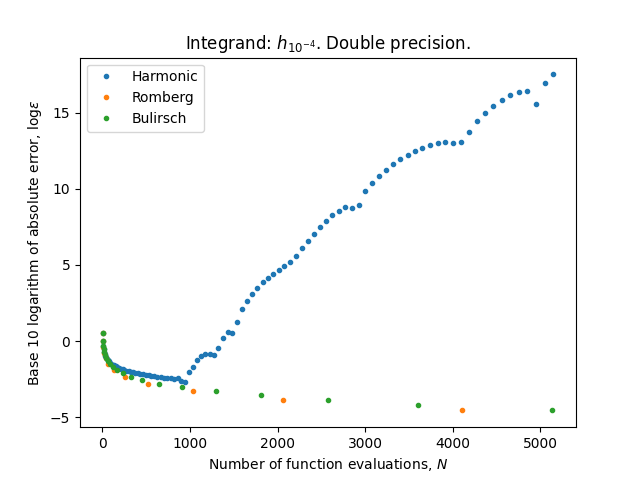
\includegraphics[scale=0.45]{diff_quot_plots/h_tenthousandth.png}
\end{minipage}
\begin{minipage}{0.45\textwidth}
\centering
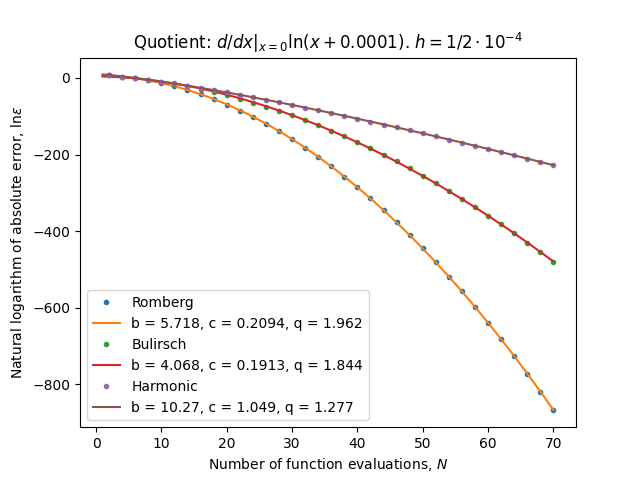
\includegraphics[scale=0.45]{diff_quot_plots/h_tenthousandth_hp_trend.png}
\end{minipage}
\end{figure}

\begin{table}[H]
    \centering
    \small
    \begin{tabular}{c|c||c|c|c|c|c|c}
Sequence & Plot & \(A\)-mean & \(A\)-var & \(c\)-mean & \(c\)-var & \(q\)-mean & \(q\)-var\\\hline
Romberg & lin-ln evals-error & \(150.3\) & \(2.443\) & \(0.2078\) & \(0.007242\) & \(1.962\) & \(0.000123\) \\
Bulirsch & lin-ln evals-error & \(59.81\) & \(6.275\) & \(0.1873\) & \(0.08379\) & \(1.851\) & \(0.001315\) \\
Harmonic & lin-ln evals-error & \(9.618\cdot 10^{5}\) & \(2.331\) & \(1.128\) & \(0.01092\) & \(1.264\) & \(0.0004176\) \\
    \end{tabular}
    \label{tab:my_label}
\end{table}

Here the same comments apply as for \(a= 1,10^{-2}\).\\

Note that the \(c\) and \(q\) parameters are independent of \(a\).

\subsection{Square root}

Now we shall consider the derivative at zero of the following function:
\[
h_a(x) \coloneqq \sqrt{a + x}, \quad a > 0.
\]

\begin{figure}[H]
\centering
\begin{minipage}{0.45\textwidth}
\centering
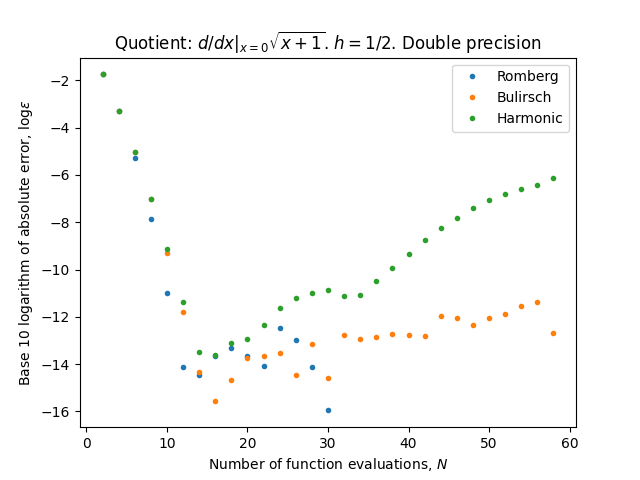
\includegraphics[scale=0.45]{diff_quot_plots/sqrt_1.png}
\end{minipage}
\begin{minipage}{0.45\textwidth}
\centering
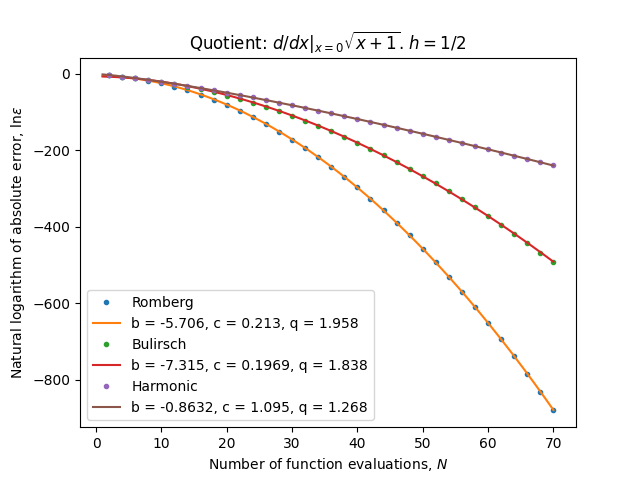
\includegraphics[scale=0.45]{diff_quot_plots/sqrt_1_hp_trend.png}
\end{minipage}
\end{figure}

\begin{table}[H]
    \centering
    \small
    \begin{tabular}{c|c||c|c|c|c|c|c}
Sequence & Plot & \(A\)-mean & \(A\)-var & \(c\)-mean & \(c\)-var & \(q\)-mean & \(q\)-var\\\hline
Romberg & lin-ln evals-error & \(0.00163\) & \(3.185\) & \(0.2109\) & \(0.009876\) & \(1.959\) & \(0.000166\) \\
Bulirsch & lin-ln evals-error & \(0.0007538\) & \(7.186\) & \(0.1925\) & \(0.09801\) & \(1.846\) & \(0.001513\) \\
Harmonic & lin-ln evals-error & \(7.958\) & \(2.102\) & \(1.159\) & \(0.008158\) & \(1.259\) & \(0.0003023\) \\
    \end{tabular}
    \label{tab:my_label}
\end{table}

In standard double precision floating point arithmetic we get down to machine level precision using any sequence. The model fits quite well for the Romberg and the Harmonic sequence but not as well for the Bulirsch sequence.

\begin{figure}[H]
\centering
\begin{minipage}{0.45\textwidth}
\centering
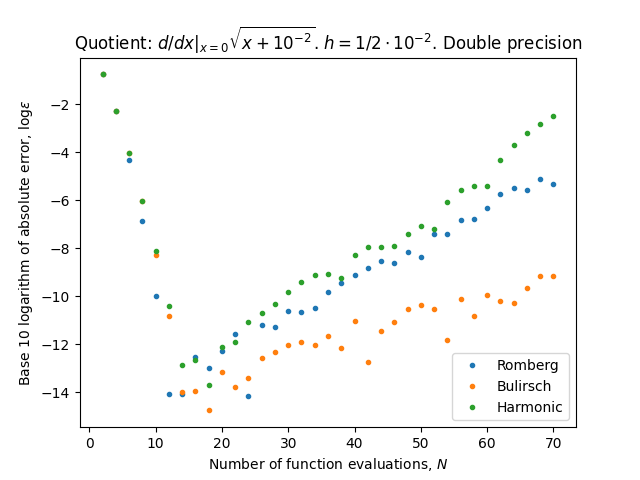
\includegraphics[scale=0.45]{diff_quot_plots/sqrt_em2.png}
\end{minipage}
\begin{minipage}{0.45\textwidth}
\centering
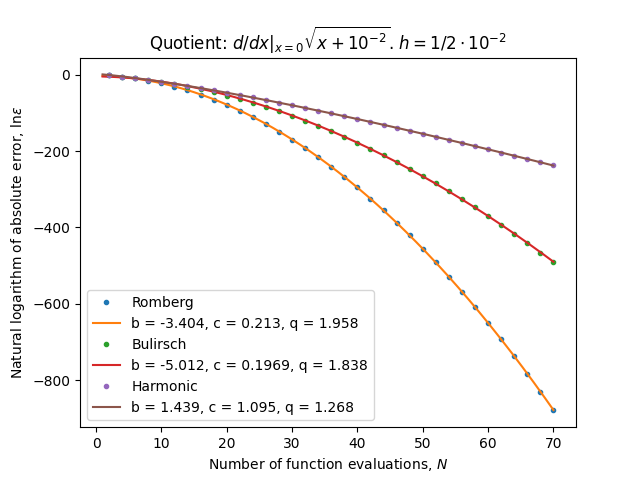
\includegraphics[scale=0.45]{diff_quot_plots/sqrt_em2_hp_trend.png}
\end{minipage}
\end{figure}

\begin{table}[H]
    \centering
    \small
    \begin{tabular}{c|c||c|c|c|c|c|c}
Sequence & Plot & \(A\)-mean & \(A\)-var & \(c\)-mean & \(c\)-var & \(q\)-mean & \(q\)-var\\\hline
Romberg & lin-ln evals-error & \(0.0163\) & \(3.185\) & \(0.2109\) & \(0.009876\) & \(1.959\) & \(0.000166\) \\
Bulirsch & lin-ln evals-error & \(0.007538\) & \(7.186\) & \(0.1925\) & \(0.09801\) & \(1.846\) & \(0.001513\) \\
Harmonic & lin-ln evals-error & \(79.58\) & \(2.102\) & \(1.159\) & \(0.008158\) & \(1.259\) & \(0.0003023\) \\
    \end{tabular}
    \label{tab:my_label}
\end{table}

Here the same comments apply as for \(a = 1\). 

\begin{figure}[H]
\centering
\begin{minipage}{0.45\textwidth}
\centering
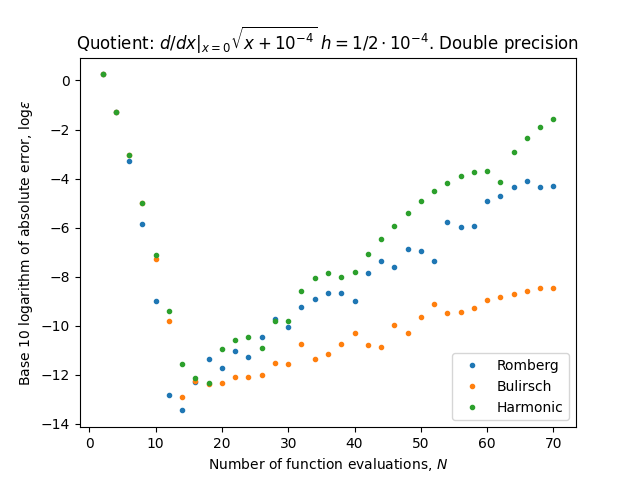
\includegraphics[scale=0.45]{diff_quot_plots/sqrt_em4.png}
\end{minipage}
\begin{minipage}{0.45\textwidth}
\centering
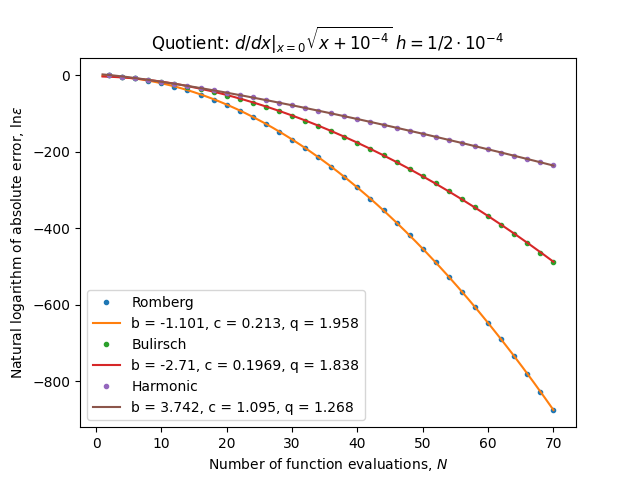
\includegraphics[scale=0.45]{diff_quot_plots/sqrt_em4_hp_trend.png}
\end{minipage}
\end{figure}

\begin{table}[H]
    \centering
    \small
    \begin{tabular}{c|c||c|c|c|c|c|c}
Sequence & Plot & \(A\)-mean & \(A\)-var & \(c\)-mean & \(c\)-var & \(q\)-mean & \(q\)-var\\\hline
Romberg & lin-ln evals-error & \(0.163\) & \(3.185\) & \(0.2109\) & \(0.009876\) & \(1.959\) & \(0.000166\) \\
Bulirsch & lin-ln evals-error & \(0.07538\) & \(7.186\) & \(0.1925\) & \(0.09801\) & \(1.846\) & \(0.001513\) \\
Harmonic & lin-ln evals-error & \(795.8\) & \(2.102\) & \(1.159\) & \(0.008158\) & \(1.259\) & \(0.0003023\) \\
    \end{tabular}
    \label{tab:my_label}
\end{table}

Here also the same comments apply.

\begin{figure}[H]
\centering
\begin{minipage}{0.45\textwidth}
\centering
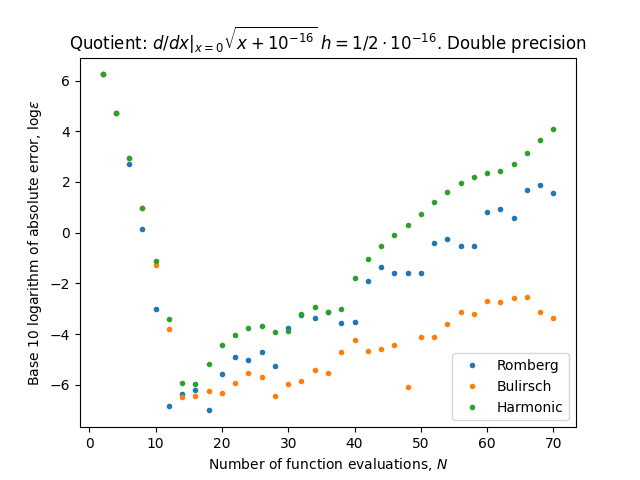
\includegraphics[scale=0.45]{diff_quot_plots/sqrt_em16.png}
\end{minipage}
\begin{minipage}{0.45\textwidth}
\centering
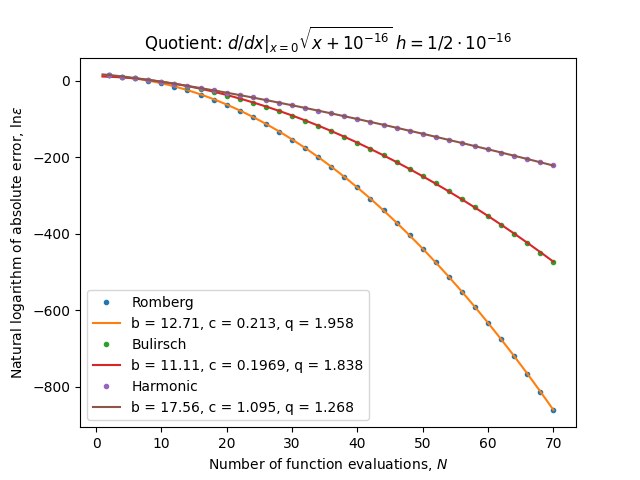
\includegraphics[scale=0.45]{diff_quot_plots/sqrt_em16_hp_trend.png}
\end{minipage}
\end{figure}

\begin{table}[H]
    \centering
    \small
    \begin{tabular}{c|c||c|c|c|c|c|c}
Sequence & Plot & \(A\)-mean & \(A\)-var & \(c\)-mean & \(c\)-var & \(q\)-mean & \(q\)-var\\\hline
Romberg & lin-ln evals-error & \(1.63\cdot 10^{5}\) & \(3.185\) & \(0.2109\) & \(0.009876\) & \(1.959\) & \(0.000166\) \\
Bulirsch & lin-ln evals-error & \(7.538\cdot 10^{4}\) & \(7.186\) & \(0.1925\) & \(0.09801\) & \(1.846\) & \(0.001513\) \\
Harmonic & lin-ln evals-error & \(7.958\cdot 10^{8}\) & \(2.102\) & \(1.159\) & \(0.008158\) & \(1.259\) & \(0.0003023\) \\
    \end{tabular}
    \label{tab:my_label}
\end{table}

And they also apply here.\\

Note that the \(c\) and \(q\) parameters are independent of \(a\).

\subsection{Smooth but not analytic function}

Now we will consider the derivate at zero of the following function:
\[
r(x) \coloneqq \begin{cases}
e^{-1/x} & \text{if } x > 0\\
0 & \text{else}
\end{cases}
\]
which is smooth but not analytic.

\begin{figure}[H]
\centering
\begin{minipage}{0.45\textwidth}
\centering
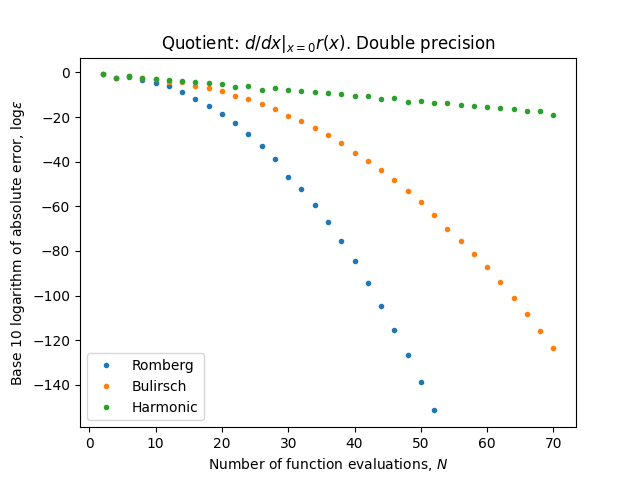
\includegraphics[scale=0.45]{diff_quot_plots/rho.png}
\end{minipage}
\begin{minipage}{0.45\textwidth}
\centering
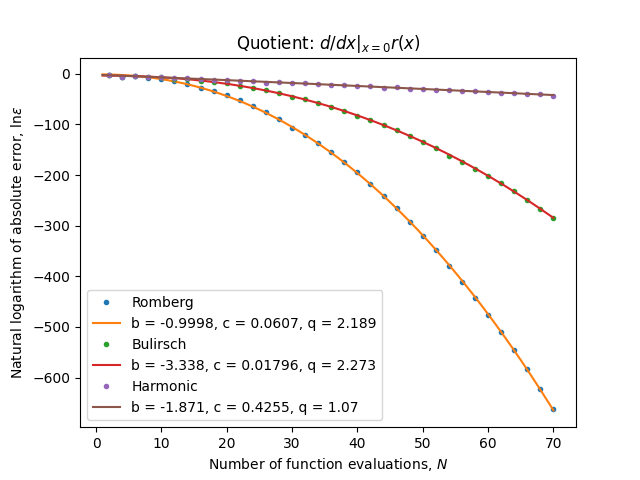
\includegraphics[scale=0.45]{diff_quot_plots/rho_hp_trend.png}
\end{minipage}
\end{figure}

\begin{table}[H]
    \centering
    \small
    \begin{tabular}{c|c||c|c|c|c|c|c}
Sequence & Plot & \(A\)-mean & \(A\)-var & \(c\)-mean & \(c\)-var & \(q\)-mean & \(q\)-var\\\hline
Romberg & lin-ln evals-error & \(6.865\cdot 10^{52}\) & \(25\) & \(0.177\) & \(2.644\) & \(2.181\) & \(0.02709\) \\
Bulirsch & lin-ln evals-error & \(4.186\cdot 10^{60}\) & \(25\) & \(0.2329\) & \(5.914\) & \(2.282\) & \(0.07529\) \\
Harmonic & lin-ln evals-error & . & . & . & . & . & . \\
    \end{tabular}
    \label{tab:my_label}
\end{table}

Here the model fits moderately well in the case of the Romberg sequence and the Bulirsch sequence but not in the case of the harmonic sequence. 

\subsection{Another smooth but not analytic function}

Now we will consider the derivative at zero of the following function:
\[
i(x)\coloneqq \begin{cases}
xe^{-1/x^2} & \text{if } x \neq 0\\
0 & \text{else}
\end{cases}
\]
which is smooth but not analytic.
\begin{figure}[H]
\centering
\begin{minipage}{0.45\textwidth}
\centering
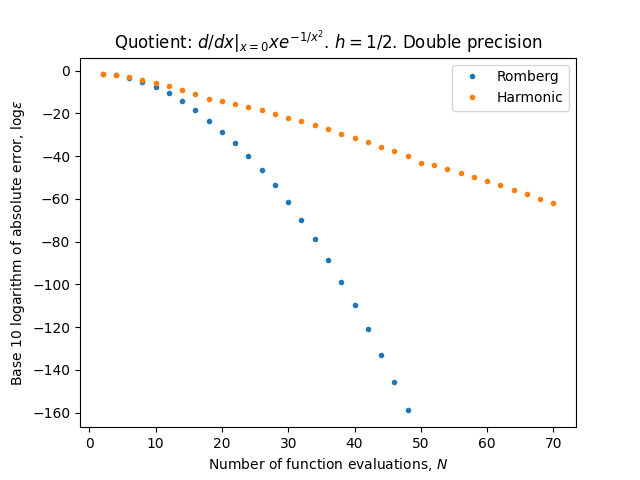
\includegraphics[scale=0.45]{diff_quot_plots/xemxm2.png}
\end{minipage}
\begin{minipage}{0.45\textwidth}
\centering
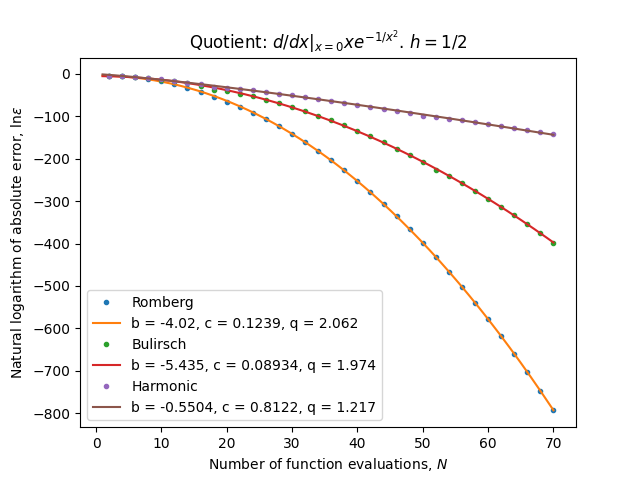
\includegraphics[scale=0.45]{diff_quot_plots/xemxm2_hp_trend.png}
\end{minipage}
\end{figure}

\begin{table}[H]
    \centering
    \small
    \begin{tabular}{c|c||c|c|c|c|c|c}
Sequence & Plot & \(A\)-mean & \(A\)-var & \(c\)-mean & \(c\)-var & \(q\)-mean & \(q\)-var\\\hline
Romberg & lin-ln evals-error & \(1228\) & \(24.39\) & \(0.1549\) & \(0.6269\) & \(2.043\) & \(0.004482\) \\
Bulirsch & lin-ln evals-error & \(1.706\cdot 10^{65}\) & \(25\) & \(1.496\) & \(7.898\) & \(1.948\) & \(0.08245\) \\
Harmonic & lin-ln evals-error & . & . & . & . & . & . \\
    \end{tabular}
    \label{tab:my_label}
\end{table}

Here the model fits fine in the case of the Romberg sequence but not in the other cases.

\subsection{Only once differentiable function}

Finally we will consider the derivate at zero of the following function which is only once differentiable at that point:
\[
j(x)\coloneqq \begin{cases}
x^2\sin\frac{1}{x} & \text{if } x \neq 0\\
0 & \text{else}
\end{cases}.
\]

\begin{figure}[H]
\centering
\begin{minipage}{0.45\textwidth}
\centering
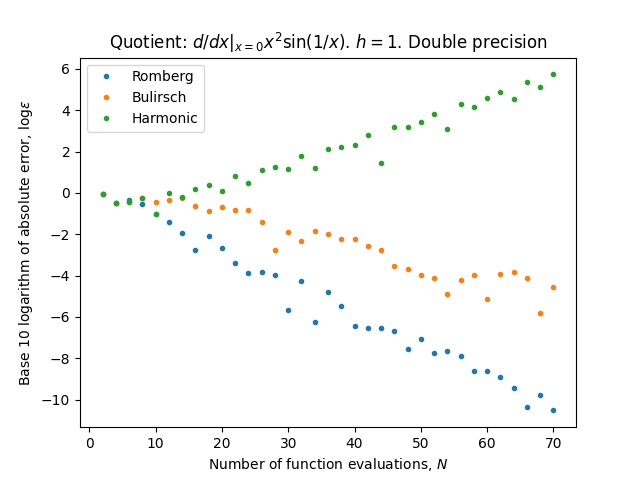
\includegraphics[scale=0.45]{diff_quot_plots/xsin.png}
\end{minipage}
\begin{minipage}{0.45\textwidth}
\centering
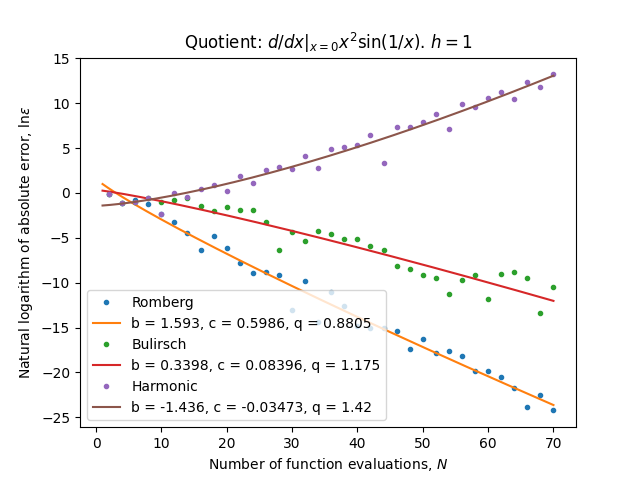
\includegraphics[scale=0.45]{diff_quot_plots/xsin_hp_trend.png}
\end{minipage}
\end{figure}

\begin{table}[H]
    \centering
    \small
    \small
    \begin{tabular}{c|c||c|c|c|c|c|c}
Sequence & Plot & \(A\)-mean & \(A\)-var & \(c\)-mean & \(c\)-var & \(q\)-mean & \(q\)-var\\\hline
Romberg & lin-ln evals-error & . & . & \(2607\) & \(2.282\) & \(4.553\) & \(3.923\) \\
Bulirsch & lin-ln evals-error & . & . & . & . & . & . \\
Harmonic & lin-ln evals-error & . & . & . & . & . & . \\
    \end{tabular}
    \label{tab:my_label}
\end{table}

Here the model simply does not fit. Note that we do not have the asymptotic expansion for the derivate here, since the function is only once differentiable.\\

The parameters from the fitting are:

\begin{table}[H]
    \centering
    \begin{tabular}{c|c||c|c|c}
        Derivative & Sequence & \(b\) & \(c\) & \(q\) \\\hline\hline
$d/dx|_{x=0}r(x)$ & Romberg & \(-0.99982\) & \(0.060703\) & \(2.189\) \\
$d/dx|_{x=0}r(x)$ & Bulirsch & \(-3.3384\) & \(0.017962\) & \(2.2735\) \\
$d/dx|_{x=0}r(x)$ & Harmonic & \(-1.8705\) & \(0.42555\) & \(1.0695\) \\
$d/dx|_{x=0}xe^{-1/x^2}$. $h=1/2$ & Romberg & \(-4.0202\) & \(0.12391\) & \(2.0616\) \\
$d/dx|_{x=0}xe^{-1/x^2}$. $h=1/2$ & Bulirsch & \(-5.4352\) & \(0.089335\) & \(1.9741\) \\
$d/dx|_{x=0}xe^{-1/x^2}$. $h=1/2$ & Harmonic & \(-0.55045\) & \(0.81216\) & \(1.2174\) \\
$d/dx|_{x=0}\sin x$. $h=1/2$ & Romberg & \(-5.3663\) & \(0.51067\) & \(1.8066\) \\
$d/dx|_{x=0}\sin x$. $h=1/2$ & Bulirsch & \(-5.1899\) & \(0.64124\) & \(1.651\) \\
$d/dx|_{x=0}\sin x$. $h=1/2$ & Harmonic & \(3.912\) & \(1.9876\) & \(1.2878\) \\
$d/dx|_{x = 0} \ln (x + 0.0001)$. $h=1/2\cdot 10^{-4}$ & Romberg & \(5.7177\) & \(0.20942\) & \(1.9619\) \\
$d/dx|_{x = 0} \ln (x + 0.0001)$. $h=1/2\cdot 10^{-4}$ & Bulirsch & \(4.0682\) & \(0.19126\) & \(1.8443\) \\
$d/dx|_{x = 0} \ln (x + 0.0001)$. $h=1/2\cdot 10^{-4}$ & Harmonic & \(10.266\) & \(1.0494\) & \(1.2768\) \\
$d/dx|_{x=0} \ln (x + 0.01)$. $h=1/2\cdot 10^{-2}$ & Romberg & \(1.1125\) & \(0.20942\) & \(1.9619\) \\
$d/dx|_{x=0} \ln (x + 0.01)$. $h=1/2\cdot 10^{-2}$ & Bulirsch & \(-0.53694\) & \(0.19126\) & \(1.8443\) \\
$d/dx|_{x=0} \ln (x + 0.01)$. $h=1/2\cdot 10^{-2}$ & Harmonic & \(5.6607\) & \(1.0494\) & \(1.2768\) \\
$d/dx|_{x=0} \ln(x + 1)$. $h=1/2$ & Romberg & \(-3.4927\) & \(0.20942\) & \(1.9619\) \\
$d/dx|_{x=0} \ln(x + 1)$. $h=1/2$ & Bulirsch & \(-5.1421\) & \(0.19126\) & \(1.8443\) \\
$d/dx|_{x=0} \ln(x + 1)$. $h=1/2$ & Harmonic & \(1.0555\) & \(1.0494\) & \(1.2768\) \\
$d/dx|_{x=0} x^2 \sin(1/x)$. $h=1$ & Romberg & \(1.5925\) & \(0.59863\) & \(0.88054\) \\
$d/dx|_{x=0} x^2 \sin(1/x)$. $h=1$ & Bulirsch & \(0.33976\) & \(0.083956\) & \(1.1751\) \\
$d/dx|_{x=0} x^2 \sin(1/x)$. $h=1$ & Harmonic & \(-1.436\) & \(-0.034733\) & \(1.4204\) \\
$d/dx|_{x=0} \sqrt{x + 1}$. $h=1/2$ & Romberg & \(-5.7063\) & \(0.21299\) & \(1.9582\) \\
$d/dx|_{x=0} \sqrt{x + 1}$. $h=1/2$ & Bulirsch & \(-7.315\) & \(0.19691\) & \(1.8379\) \\
$d/dx|_{x=0} \sqrt{x + 1}$. $h=1/2$ & Harmonic & \(-0.86323\) & \(1.0951\) & \(1.2682\) \\
$d/dx|_{x=0}\sqrt{x + 10^{-2}}$. $h=1/2\cdot 10^{-2}$ & Romberg & \(-3.4037\) & \(0.21299\) & \(1.9582\) \\
$d/dx|_{x=0}\sqrt{x + 10^{-2}}$. $h=1/2\cdot 10^{-2}$ & Bulirsch & \(-5.0125\) & \(0.19691\) & \(1.8379\) \\
$d/dx|_{x=0}\sqrt{x + 10^{-2}}$. $h=1/2\cdot 10^{-2}$ & Harmonic & \(1.4394\) & \(1.0951\) & \(1.2682\) \\
$d/dx|_{x=0}\sqrt{x + 10^{-4}}$ $h=1/2\cdot 10^{-4}$ & Romberg & \(-1.1011\) & \(0.21299\) & \(1.9582\) \\
$d/dx|_{x=0}\sqrt{x + 10^{-4}}$ $h=1/2\cdot 10^{-4}$ & Bulirsch & \(-2.7099\) & \(0.19691\) & \(1.8379\) \\
$d/dx|_{x=0}\sqrt{x + 10^{-4}}$ $h=1/2\cdot 10^{-4}$ & Harmonic & \(3.7419\) & \(1.0951\) & \(1.2682\) \\
$d/dx|_{x=0}\sqrt{x + 10^{-16}}$ $h=1/2\cdot 10^{-16}$ & Romberg & \(12.714\) & \(0.21299\) & \(1.9582\) \\
$d/dx|_{x=0}\sqrt{x + 10^{-16}}$ $h=1/2\cdot 10^{-16}$ & Bulirsch & \(11.106\) & \(0.19691\) & \(1.8379\) \\
$d/dx|_{x=0}\sqrt{x + 10^{-16}}$ $h=1/2\cdot 10^{-16}$ & Harmonic & \(17.557\) & \(1.0951\) & \(1.2682\) \\
$d/dx|_{x=0}e^x$ & Romberg & \(-2.408\) & \(0.41106\) & \(1.8479\) \\
$d/dx|_{x=0}e^x$ & Bulirsch & \(-2.9068\) & \(0.48137\) & \(1.703\) \\
$d/dx|_{x=0}e^x$ & Harmonic & \(4.7175\) & \(1.5509\) & \(1.3212\) \\
    \end{tabular}
    \caption{Optimal parameters by test case}
    \label{tab:my_label}
\end{table}

Excluding the computation of \(d/dx|_{x=0}x^2\sin 1/x\), the model fits exceptionally. We always get fast convergence except when computing \(d/dx|_{x=0}x\sin 1/x\) and extrapolation with the harmonic sequence. Excluding this case, we always get almost down to machine level precision when using double precision arithmetic, using any extrapolation sequence. It is worth noting that \(x\sin 1/x\) is only once differentiable at \(0\) so we do not have the asymptotic expansion for its derivative at \(0\). The Romberg sequence performes best and the harmonic sequence worst, in all cases.\\